\documentclass[sigconf,screen,9pt,natbib=false]{acmart}
\usepackage[style=ieee, sorting=nyt, urldate=long, date=long, backend=biber]{biblatex}
\addbibresource{references.bib}
% Flag to disable all editing macros and make the document ready for
%  submission.
\newif\ifEditMode

% Editing mode.
\EditModetrue
% % Submission mode.
% % The `submission' mode merges certain comments and edits, and removes some
% % other notes, TODOs and remarks. For more details, refer to the `reviewing
% % macros' in the `vusec.sty' file.
% \EditModefalse

\usepackage{vu}
\usepackage{frontmatter}
\usepackage{aliases}
\usepackage{codestyle}
\usepackage{tikz}

\begin{document}

%% Thesis title.
\newcommand{\thesistitle}{High performance FFI in Julia: A case study of the FFI landscape}

%% Author information.
%% (Used in a couple of places, so it's better to define them in one place.)
\newcommand{\thauthor}{Kai Erik Niermann}
\newcommand{\thauthorid}{2720905}
\newcommand{\thauthoremail}{k.e.niermann@student.vu.nl}
\newcommand{\thauthoraff}{Vrije Universiteit Amsterdam}


%% Thesis type.
%% Valid values are `vubachelor', `csmaster', `pdcsmaster', and `litstudy'.
%%
\thtype{vubachelor}

%% Thesis title.
\thtitle{\thesistitle}

%% Paper/thesis author.
\thauthname{\thauthor}

%% First supervisor.
\thsvfirst{Atze Van der Ploeg}{Assistant Professor}

%% Daily supervisor.
\thsvdaily{Atze Van der Ploeg}{Assistant Professor}

%% Second reader.
\thrdrsecond{Verano Merino}{Assistant Professor}

%% Attach customize front matter.
\addfrontmatter{}

\title{\thesistitle}

\author{\thauthor}
\affiliation{
  \institution{\thauthoraff}
  \city{Amsterdam}
  \country{The Netherlands}
}
\email{\thauthoremail}

\begin{abstract}

\TODO{Your Master Thesis has to be written in English and should follow the ACM style (see the \href{https://www.overleaf.com/latex/templates/vu-is-research-thesis/kkymstmdhrns}{Overleaf template}). We also suggest a \textit{structured abstract} following the structure below.}

\noindent \textit{Context}. 
\TODO{Write this at the end}

\noindent \textit{Goal}. 
\TODO{Write this at the end}

\noindent \textit{Method}. 
\TODO{Write this at the end}

\noindent \textit{Results}. 
\TODO{Write this at the end}

\noindent \textit{Conclusions}. 
\TODO{Write this at the end}

\TODO{As a very rough indication, the final thesis report typically entails, excluding appendixes, between 10 and 30 pages, with an average of 15 pages. The large variation depends on many variables including the specific field, project nature, and context. We advise to ask your supervisor if you should consider which number as a reference.}

\end{abstract}

\maketitle

\pagestyle{plain}
\pagenumbering{arabic}

\section{Introduction} \label{s:intro}

\TODO{
This section includes the context and motivation behind the work, explicitly or implicitly highlights the main research question(s), provides a high-level explanation of the solution, and describes the contributions.}

\TODO{Context, motivation, research question asds, and original contribution could be organized in subsections.}

\begin{figure}[!h]
    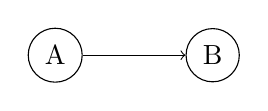
\begin{tikzpicture}
  \node[draw, circle] (a) at (0,0) {A};
  \node[draw, circle] (b) at (2,0) {B};
  \draw[->] (a) -- (b);
\end{tikzpicture}

\end{figure}

% briefly talk about physically based rendering 

% talk about the relevance of performance and optimizations 

% talk about the motivation behind the comparative analysis
    % what is the general idea behind the analysis
    % what are the goals of the analysis
    % what are the expected outcomes of the analysis
    % what isthe importance of this

% give some of the research questions that will be answered in the analysis

% give a brief overview of the methodology used in the analysis




% ---------- templates for figures ----------------------- 

% \begin{figure}[bh]
%     %% The macro `\onecolgrid' is defined in `vusec.sty'
%     %% NOTE: The suffix "./figures/" is implicitly included for this relative path.
%     \includegraphics[width=\onecolgrid]{cache-by-app}
%     %% Labels should immediately follow caption, to keep latex quiet.
%     \figcap{Simple one-column figure. Please include a brief explanation or takeaway.}\label{fig:1col}
% \end{figure}

% \begin{figure*}[th]
%     %% The macro `\threecolgrid' is defined in `vusec.sty'
%     \begin{subfigure}[t]{\threecolgrid}
%         %% NOTE: The suffix "./figures/" is implicitly included for these relative paths.
%         \includegraphics[width=\linewidth]{three-col/speed_index}
%         \sfigcap{}\label{fig:3col-a}
%     \end{subfigure}
%     \begin{subfigure}[t]{\threecolgrid}
%         %% NOTE: You do not have to mention the extension.
%         %% (The example figures are in PDF format.)
%         \includegraphics[width=\linewidth]{three-col/plt_ranks_diff}
%         \sfigcap{}\label{fig:3col-b}
%     \end{subfigure}
%     \begin{subfigure}[t]{\threecolgrid}
%         \includegraphics[width=\linewidth]{three-col/mimes}
%         \sfigcap{}\label{fig:3col-c}
%     \end{subfigure}
%     %% Labels should immediately follow caption, to keep latex quiet.
%     \figcap{Generate clear and beautiful figures (in PDF) that can be rendered side by side while still being easy to read and interpret. Choose colors wisely from the colorbrewer2.org website.}\label{fig:3col}
% \end{figure*}

% \begin{table}[hb]
%     \centering
%     \tabcap{A simple table describing the characteristics of a data set or the results of an experiment}\label{tab:sample}
%     \taburulecolor{black!45}
%     \begin{tabu}{c|c|r|r|r|r}
%         \toprule
%         \multirow{2}{*}{\thead{Char.}} &
%             \multirow{2}{*}{\thead{\#samples}} &
%             \thead{Count} &
%             \multicolumn{3}{c}{\thead{Perf. Score}}\\
%         &
%             &
%             \thead{of items} &
%             \thead{X} & \thead{Y} & \thead{Z} \\
%         \midrule
%         \stress{P}
%             & 214 & 56 & 9 & 23 & 24 \\
%         \stress{Q}
%             & 117 & 27 & 7 & 10 & 10 \\
%         \stress{R}
%             & 222 & 11 & 6 & 4 & 1 \\
%         \stress{S}
%             & 187 &  9 & 1 & 6 & 2 \\
%         \stress{T}
%             & 180 & 16 & 7 & 5 & 4 \\
%         \bottomrule
%     \end{tabu}

% \end{table}

 

\section{Background \& Related work}\label{s:background}

To further gain insights into this world of interoperability I thought it best to continue on with the idea I had of rewriting a component in different languages and then applying some system of interoperability. Decomposing this idea into concrete steps we can develop a rough design of how this study will be conducted.
\begin{enumerate}
    \item Literature review \& Background
    \begin{enumerate}
        \item Review current landscape of language interoperability
        \item Choose suitable libraries to explore our specific use case
    \end{enumerate}
    \item Implementation
    \begin{enumerate}
        \item Profile the Julia application to extract the most performance intensive piece of code
        \item Rewrite this piece of code in different languages, preferably ones which have very different execution models
        \item Write some type of glue layers utilizing the chosen libraries to enable this interoperability
    \end{enumerate}
    \item Analysis \& Development
    \begin{enumerate}
        \item Understand how the type systems of these different languages interact, especially considering types beyond primitives
        \item Profile the programs for all given languages to understand the performance impacts
        \begin{enumerate}
            \item Understand the underlying nature of the performance impacts and how they relate to differences in execution models
        \end{enumerate}
        \item Understand how interop libraries are designed and enable communication between languages
        \begin{enumerate}
            \item Attempt to develop certain solutions for any limitations encountered
        \end{enumerate}
    \end{enumerate}
\end{enumerate}

\subtitle{Foreign Function Interface (FFI)}

FFI is a generic term which describes any implementation which enables a piece of code written in one language to call functions written in another. As the name implies these implementations usually provide some interface; that is, abstractions; which enable a programmer to make calls into some binary compiled into some target language differing from the source. In practice FFI can be thought of as existing on two layers, the Application Binary Interface (ABI) level and the Application Programming Interface (API) level. The ABI level describes some common standard for how to compile source code into machine code. The API level then describes the corresponding high-level counterpart which comes in the form of libraries which expose means of working with this underlying shared ABI as to enable communication in a shared low level standard. By far the most common ABI which many languages can compile to and by extension have interoperability with is the C ABI.\@ One slight tangent, naturally when we talk about an ABI we are referring to machine level concepts, which is to say that while its become the de facto standard to say `C ABI' the underlying standard's we are talking about are the platform specific ABI standards which C compilers correspond to. It's just more straightforward to say there is a universal `C ABI' as superficially this is more or less accurate.

\begin{minted}[
    frame=lines,
    fontsize=\footnotesize, 
    linenos,
    numbersep=5pt,
    xleftmargin=5pt
]{C}
// mylib.c
#include <stdio.h>

void greet(const char* name) {
    printf("Hello, %s!\n", name);
}
\end{minted}

\begin{minted}[
    frame=lines,
    fontsize=\footnotesize, 
    linenos,
    numbersep=5pt,
    xleftmargin=5pt
]{julia}
ccall((:greet, "mylib"), Cvoid, (Cstring,), "World")
\end{minted}

\begin{minted}[
    frame=lines,
    fontsize=\footnotesize, 
    linenos,
    numbersep=5pt,
    xleftmargin=5pt
]{rust}
#[link(name = "mylib")] 
extern "C" { fn greet(name: *const c_char); }

fn main() { 
    let name = "World"; 
    let c_name = CString::new(name).expect("CString::new failed"); 
    unsafe { 
        greet(c_name.as_ptr()); 
    } 
}
\end{minted}

\begin{minted}[
    frame=lines,
    fontsize=\footnotesize, 
    linenos,
    numbersep=5pt,
    xleftmargin=5pt
]{python}
mylib = ctypes.CDLL('./libmylib.so')

mylib.greet.argtypes = [ctypes.c_char_p]  
mylib.greet.restype = None                  

name = b"World"  
mylib.greet(name)
\end{minted}

One critical thing to observe is in all instance we must ensure the FFI boundary method and its arguments conform to the memory layout of the target language as specified by the ABI.\@ Since string types for example generally have different underlying representations depending on the language here we must ensure the string has the form of a C-string, that is its a basic pointer to an array of characters \textit{char*}.

This in turn limits FFI boundary methods by the syntax and underlying ABI of our target language. For example, as C has no generics, we cannot utilize a generic method as an FFI boundary despite generics existing in our source language and Rust being compatible with the C ABI.\@

\begin{minted}[
    frame=lines,
    fontsize=\footnotesize, 
    linenos,
    numbersep=5pt,
    xleftmargin=5pt
]{rust}
extern "C" { 
    fn add<T>(a: T, b: T) -> T; 
}
\end{minted}

Stated differently FFI boundary method signatures must mirror those of the target language. We can create some flexibility here by abstracting the boundary utilizing wrappers; commonly macros; which make defining the boundary closer to that of the source language while implicitly ensuring that the actual underlying boundary is valid, an example of this is the \texttt{@ccall} macro in Julia.

But this doesn't really address the underlying issue that our FFI boundary is limited by the target language. 

\subsection{Application Binary Interface (ABI)}

ABI stability is a key factor to understanding the current landscape of not only interoperability between languages but also within different versions of languages themselves. As the name implies the stability of an ABI refers to its specification, that being how a compiler generates machine code, being stable or unchanging. An ABI being `fully stable' implies that all aspects of its specifications will not change with any future modification of its execution system (JIT compiler, AOT compiler, etc.). One of the primary reasons for so many languages having interop with C is due to the fact that it has full ABI stability, thus there exist essentially a promise that a compiler can always generate the same machine code for a given source language that conforms to the defined C ABI standard knowing this will never some day break due to changes in C's calling conventions, memory layout, etc. 

The other side of this is ABI instability, most languages currently have what could be considered partial ABI stability. What this means in practice is that most languages have some execution system which generates machine code, commonly this version or a set of versions have a common ABI.\@ Within this set of versions there exists stability, meaning shared library calls; which are reliant on ABI stability; can function with any other languages capable of producing machine code which conforms to this ABI.\@ Though across different ABI's this communication breaks down as we no longer have a homogenous standard generating the machine code but conflicting and often incompatible standards. 

This nature of partial stability in the ABI's of most languages creates one of the primary limitations to language interoperability with FFI, due to the rather complex and to an extent controversial nature of having an ABI which is both fully specified and consistent across versions there are not alot of languages which have this and by extension not alot of compilers which chose to implement an ABI for this. Furthermore there is the point that if for some set of languages there is an existing C ABI already implemented, this in turn implies we have communication between these two languages with the common language taking the form of the C ABI.\@ It should be clarified that while interop in many languages occurs with the C ABI as the basic common ground. 

\subsection{C-ABI and Interop in practice}

To describe how interop utilizing the C ABI actually plays out in practice lets express two arbitrary languages as $L_1$ and $L_2$. In the case of primitives the generated machine code usually produces matching layouts, thus little additional work is involved beyond defining the FFI boundaries in both languages. As we start getting to more complex types we start wanting to pass more complex things across the FFI boundary that might not have as straightforward of a representation in C we run into the first issue with pure C ABI based interop. This being that it leads to considerable manual specification and redefining languages specific syntax, otherwise called marshalling or boxing through the FFI boundary and in turn unmarshalling in the target language. Additionally we must ensure that the representation of our type in $L_1$ matches that in $L_2$ which for a large library could mean having to manually specific all types such that we establish a mirrored relationship; while this is somewhat obvious that it has to happen the manual nature of it would be less then desirable in the case of very large libraries we wish to interop with.

To address these issues of having to manually box everything such that it is compatible with the C ABI various language features and libraries exist as abstractions to enable more seamless and simplified interop between languages. The common features with these interoperability abstraction systems are usually automatic binding generation through parsing and implicit boxing and unboxing of complex types that cant be trivially passed through the FFI boundary. Examples of this are Rusts CXX library or the way Swift implemented interop as a direct part of its compiler.

Through these abstractions interop between many languages has become a mostly trivial task, in that most of the manual activities are now generally automated in one way or another, though as stated before due to the fact that this is all ultimately still working through the C-ABI (or some slight modification of it) we are still very much limited in the things we can actually pass between languages. Though these limitations are generally not large enough to really discourage the usage of FFI as the primary means of interop. 

So to briefly summarize we can see that FFI generally relies on a common denominator ABI between languages; often the C ABI;\@ and a set of tools to automate any manual boxing and unboxing such that the developer can; for the most part; simply define a boundary in both languages and use said boundary as if it were a regular call. An important final consideration with these FFI systems is how optimization works across language boundaries. Since the methods of shared libraries are only resolved at link time no optimizations except LTO can occur. The shared object file from the target language has optimizations applied from its own compiler then depending on if the compiler has Link Time Optimization (LTO) implemented we can optimize the whole program across the language boundary, otherwise no optimizations occurs across the language boundary.

\subsection{WebAssembly (WASM)}

WASM offers an interesting insights into how language interop is developing on the web. First announced in 2015 and then released in 2017 WASM is a byte-code format designed to be executed within web-browsers using stack-based Virtual Machines (VM) though has now also been implemented to run both via AOT and JIT compilers. The WASM specification was designed by the World Wide Web Consortium (W3C) but has various compiler implementations by different groups.  WASM when used as a compilation target for other languages not only allows potentially arbitrary languages to run on the web, but through its ABI also allows for another common denominator of communication. To understand the state of its ABI we have to examine the different compiler toolchains that target WASM.\@ Currently the major ones are 

\begin{table*}[ht!]
\centering
\begin{tabular}{|l|p{15cm}|}
\hline
\textbf{Compiler/Toolchain} & \textbf{Description} \\ \hline
Emscripten & This was the first project to define a POSIX compliant ABI for WASM, though as of 2020 at least it is not stable. \\ \hline
Cheerp & Seem to support WASI-WASM as a target for the compiler. Inherently has interop with JS because it literally compiles to JS uses \href{https://github.com/leaningtech/ts2cpp/}{ts2cpp} for creating C++ interfaces from TS types. \\ \hline
WASI & A subgroup of the WASM community group which is aiming to define a set of APIs and a canonical WASM ABI, currently the actual implementation of this specification comes in the form of:
\begin{itemize}
    \item \href{https://github.com/wasienv/wasienv}{Wasienv}\cite{Akbary2023wasienv} which can compile Swift and C++ to wasm conforming to the WASI standard.
    \item \href{https://github.com/WebAssembly/wasi-sdk}{wasi-sdk}\cite{Gohman2024WebAssembly} which seems to be some more low level compiler for wasi, i think the like backend, so you just need to implement the frontend for specific languages.
    \item \href{https://wasmtime.dev/}{wasmtime}\cite{wasmtime_intro} another wasm runtime which also has WASI as a target specification it seems.
    \item \href{https://github.com/singlestore-labs/wasix}{wasix}\cite{wasix} compatibility layer to make WASI POSIX compliant when built with the WASI SDK.
    \item \href{https://github.com/bytecodealliance/cargo-wasi}{wasm32-wasi}\cite{cargo-wasi} seems to be a frontend for Rust again using WASI.
\end{itemize}
WASI with the component model seems to have the most thoroughly documented ABI. \\ \hline
GoJS & Not much info on this, just seems that a \href{https://tinygo.org/}{go compiler}\cite{Ayke2024tinygo} has wasm as a target. \\ \hline
\end{tabular}
\caption{Major WASM Compiler Toolchains and Their Descriptions}
\label{table:wasm_compilers}
\end{table*}

What we can understand from this is that it seems WASI will be the ABI to which wasi-wasm will be the likely target most compilers aim to ultimately achieve, furthermore WASI seems to aim for stability with its canonical ABI, which could suggest that we might see a new common standard of interoperability, especially as wasm compilers evolve. One distinguishing feature of specifically WASI's canonical ABI is development of the \textbf{component model}, the component model refers to type definitions written in \textit{WASM Interface Type} (WIT), which is an interface description language (IDL) used to express interface; that is, types and functions; in a language agnostic manner\cite{WebAssemblyComponentModel}. From the defined WIT code we can generate the corresponding bindings in our language thus mitigating the need for any type-shenanigan's in the case of interop since our generated bindings will by default be compatible with the ABI.\@ It should be noted that as the documentation specifies WIT implements contracts, that is similar to how an \textit{extern} block expresses a function which must be ABI compatible so to do the generated bindings from the WIT code all inherently imply compatability with the underlying ABI.\@ 

Thus if you have say some library compiled to wasi-wasm which utilizes the component model to specify the API you can in turn use the library specification to generate ABI compliant bindings for your source code, then use a wasi-wasm compiler and have full cross-language interoperability without the need for any complex wrapper libraries. Though once again here we are limited by the expressiveness of the component model and corresponding ABI, meaning that if a library wants to make something available for use externally it has to conform to the component model thus potentially limiting certain language specific features for a cross language setting. Unless similarly to the C ABI we adjust the compiler to support these language specific features and in turn break compatibility with the ABI.\@ 

\subsection{Binding generator designs}

It should be clarified that in the previous instances of interop I for the most part avoided mentioning the exact details of how different type systems are mapped between languages. In the context of FFI based interop there are two key considerations in regards to types one must consider, that being the kind of type we are bridging and the parameter-passing strategy.

To talk about the parameter passing strategy we have to first talk about how types are implemented to begin with. Usually the choice of parameter-passing is closely tied to the underlying execution method of a language. Managed languages and especially high level ones generally make the choice of implementing types through boxing which in turn means they implement the call by sharing parameter passing strategy; which means that types which are cheap to copy are passed by value (boxed or not) and types which arent are passed in a way where reassignments do not affect the caller but mutations are reflected in the caller. Languages generally termed `safe' which implement some form of memory usually implement both call by value and call by reference leaving it up to the user to decide which to use for what type through certain operator choices. Finally languages which do allow memory management as a native part also usually expose pass by address where you pass a pointer which you can then dereference to use in the calling function. 

A common pattern we can spot with the design of languages is the approach that primitives; regardless of implementation; are copied, and usually user-defined types or just anything which would be unreasonably to copy can either be passed by reference by the programmer or is implicitly done so as the implemented parameter-passing strategy. One notable strategy which has gained particular notiaraiety in recent years in the case of pass by value is if you move the type by copying or by destroying it. Rust; similar to most other languages copies small stack allocated types; but in the case of anything heap allocated as a part of the rust borrow checker such values are destructively moved. When we talk about a move as opposed to a copy the simple idea is usually just that as opposed to copying heap allocated data when we pass something by value we instead simply; through some mechanism; invalidate the source object and create a new object which points to this underlying heap allocated data. The destinction being that we in essence only ever create a new owner for the heap data as opposed to creating a new owner with their own copy of the data. 

Currently the two prominant implementations of these dynamics come from C++ with move constructors and Rust with its borrow checker. The main distinguishing feature of these implementations is that in principle with C++ the moved-from object is nullified but left in a valid state such that a destructor can be called on it when it goes out of scope, whereas in Rust the old moved-from object is in an invalid state and would raise errors if used after a move, Swift has similarly implemented destructive move since v5.9 with the introduction of the \texttt{consume} operator. How long a particular variable exists from the point of creation to it being either destructively or non-destructively moved is generally referred to as the variables lifetime. As Rust has destructive move semantics as a central feature of its borrow-checker and does not use Garbage Collection (GC) it relies on either implicit (via elision) or explicit lifetime annotations as a means of conveying how long a specific variable persists for usage before being destroyed. To then brielfy summarize, we end up with essentially 3 variants of how languages pass paramaters, we either copy, pass some type of reference (either with shared semantics or not), or we give ownership. 

A good question then becomes how do we effectively implement parameter-passing in an interoperability setting. The most obvious starting point would be that; just as we want for programming languages; types which are cheap to copy should be copied. Most languages do this by defining usually some set of ABI (usually C) compatible primitive datatypes. As most languages implement a decent set of primitives in a roughly similar fashion passing these by value across a shared ABI is generally not too complex and usually forms the initial implementation of most FFI based interop systems. Once we move past basic stack allocated primitives we start to get into the realm of some complexity. A common type introduced to new programmers after primitives is the struct. Or more abstractly speaking the user defined type (UDT). UDT's can broadly be described as types which generally group some set of more fundamental types along with sets of operations that can be prefromed on these types. Both of these attributes of UDT's are usually implemented as some form of property of our type. 

As FFI based interop generally concerns some low level intermediary an important question which has to be asked is how do different languages represent object properties at a low level. Enumerating all the different object representation models for all languages would be somewhat out of scope and meaningless so I will simply describe the abstract approaches which are generally taken. On a high level we can distinguish broadly between two types of objects; direct objects and indirect objects. Direct objects here refers to objects which are represented directly in memory and whos property access usually translate to basic pointer offset computations. Direct objects usually exist in most statically typed, AOT compiled languages generally denoted with the keyword \texttt{struct} or \texttt{class} as a convention. When it comes to bridging direct objects the aim is firstly that property accesses resolve to the same memory location and that the type of the property, or more specifically the underlying memory has some analogue in the target language.

In cases where the memory does not align we start to encounter different implementation approaches one can take. The most trivial approach would be to simply expose property getters across the FFI boundary and then handle the property types as necessary. Though if we take this approach at face value its simply not feasable especially for large scale API's in some foreign language we wish to use in a different target. 

- memory management    
    - this is a big thing how we deal with memory management and variable lifetimes 
        - dying when it goes out of scope 
        - dying when its destroyed (destructive move)
        - dying when its not used anymore (statically checked)
    - so the question becomes how do you reconcile differences in memory management
        - annotations seems to be a common approach 
            - crubit lifetime annotations (uses like clangs annotations i think) based on clangs lifetime bounds i think
                - they run static lifetime analysis on the c++ code basically they try to mirror Rust's lifetime system 
            - clang lifetime bound annotation
    - the main question is how do you deal with the lifetimes of objects 
        - value types : copying 
            - Here when passing things across the language boundary and between things in the target language we copy the object
            - Obviously mutations to this object are not reflected in the source language 
        - reference types
            => so by this we mean pointers or references to objects 
            - clearly here mutations will be reflected in the source language 
            - types of references 
                - raw pointers (*)
                - reference types (&)
                - "safe" pointer types (e.g. shared_ptr)

% binding / blue code implementations 
% - binding 
%     - wrappers that allow you to use something in a target language
% - binding construction (metadata phase)
%     - since we need some representation of the types in both languages 
%     - so the question is how do we generate these bindings 
%     - automatically 
%         - we parse the headers 
%             => frontend compiler tools (clang AST parser)
%             - alot more difficult to work with as we only need a very restricted portion of the ast, that is we just need the header information 
%             => manually implemented header parsers (crubit I think)
%             - easier to implement and apply in our binding generation tool but also means we have to basically reimplement existing frontend tooling
%         - we use code reflection 
%             => languages which implement strong reflection systems (AKA python)
%             - reflect on the types and extract runtime type metadata to generat bindings for target language 
%             -! issues: 
%                 - reflection is not supported in many languages 
%                 - many languages arent even designed to ever really accomodate it properly, 
%                 - additionaly reflections systems can potentially not provide enough or just not the right information needed
%                 - examples: Python, Java, C#
%     - manual specification 
%         - we can manually specificy the bindings
%         => example: Boost.python (pybind11, CxxWrap) use manual specifications and then code generation from the specifications 
%         -! issue: obvious fact that it requires manual specification
%         -! benefit: we dont need to work with parsers at all, i mean idfk im not gonna enmerate on everything

% - binding generation 
%     - once we have the type metadata how do we generate bindings 
%     - depends on language compatability 
%         - similar languages 
%         => bindings form minimal interfaces, we might only need to apply slight transformations to the source type so its representable in the target language 
%             - sometimes even no transformations at all but I think rarely
%             - sometimes we have cases where compilers are like kinda designed with multiple languages in mind 
%                 - Cython compiler can generate C code

%         - disimilar languages 
%         => bindings are generally more complex in nature, here to my knowledge there are kinda two ways to implement things 
%             - connected glue code layers 
%             => this is what most implementations do, in that the generated bindings often dont really appear as idiomatically mirrored types but instead as clear wrappers which expose certain functionality that can be bridged 

%             - disconnected glue code layers 
%             => this seems to be alot less common, here the glue code layer is essentially hidden in that you have idiomatically mirrored types, naturally things are still restricted by what the library can mirror but for all types which can be bridged for the user end everything is completely exposed 
%             - in this case the glue code layer instead of consiting of wrappers which hold memory it instantates those mirrored types which its capable of briding

% - when do we do all of this 
%     => preprocessor tool based generation
%     - most tools have this as a separate build step usually reliant on some library to preform the binding generation, so this is usually a preprocessing step that happens before the actual execution of the application 
    
%     => static compiler based generation 
%     - sometimes compilers themselves have interoperability baked in 
%         - swiftc : swift compiler has clang embedded and has header parsing built in, this essentially forms a disconnected glue code layer in that it allows us on the developer level to use any bridagble type in an idiomatically mirrored fashion
    
%     => runtime based generation 
%     - seems to be generally effective in languages focused on dynamism 
%     - some tools aim to have runtime binding generation, only two instances i can find are javacpp and cppyy 
%         - a key benefit of this is that you can utilize runtime information to dynamically work with constructs exposed by the API 
%         - more or less just useful with monomorphization but also other stuff i think
         
\subsection{Generic types and metaprogramming models}


\subsection{Metaprogramming in the wild}
\section{Research Strategies and Research Methods}\label{s:method}

\TODO{
In this section, you would provide a description of: the research strategy (well-formulated and justified); the data collection and data analysis methods; and a clear link explaining how research strategy and methods are suitable to answer the research question(s). Include a figure providing a overview of the whole thesis in terms of research strategies/methods, RQs, inputs and outputs. An example is given in Figure \ref{fig:method}.
}

\lipsum[1-3]

\begin{figure*}[ht!]
    \includegraphics[width=0.9\textwidth]{figures/study-design.png}
    %% Labels should immediately follow caption, to keep latex quiet.
    \figcap{Overview: Research strategy, research methods and results. [Credits: illustration with Diagram.net]}\label{fig:method}
\end{figure*}

\lipsum[1-3]

\section{Implementation}\label{s:implementation}

% \begin{figure*}[ht!]
%     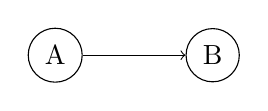
\begin{tikzpicture}
  \node[draw, circle] (a) at (0,0) {A};
  \node[draw, circle] (b) at (2,0) {B};
  \draw[->] (a) -- (b);
\end{tikzpicture}

%     \figcap{System architecture of multi-language PBR renderer.}\label{fig:main_interface}
% \end{figure*}

\subsection{Part 1: We have a problem}



\subsection{Part 2: Designing a solution}


\subsection{Part 3: How well does it work?}
\section{Discussion}\label{s:discussion}


\TODO{
Here you put your results in context (possibly grouped by research question). Usually, this section focuses on analyzing the
implications of the proposed work for current and future research and for practitioners.
}


% \lipsum[1-8]

\section{Related Work}\label{s:related}


\TODO{
Describe here scientific papers similar to your thesis work, both in terms of goal and methodology. One paragraph for each paper (we expect about 5-8 papers to be discussed). Each paragraph contains: (i) a brief description of the related paper and (ii) a black-on-white description about how your work differs from, or overlaps with, the related paper, hence emphasizing the novelty contributed by this thesis. You may place this section immediately after the Background section, if necessary.
}


\lipsum[14-17][4-8]


\input{sections/conclusion}

% \bibliographystyle{ACM-Reference-Format}
\printbibliography

\end{document}


%%% Local Variables:
%%% mode: latex
%%% TeX-master: t
%%% End:
